\documentclass[12pt,twoside]{article}

%%%%%%%%%%%%%%%%%%%%%%%%%%%%%%%%%%%%%%%%%%%%%%%%%%%%%%%%%%%%%%%%%%%%%%%%%%%%%

% Definitions for the title page
% Edit these to provide the correct information
% e.g. \newcommand{\reportauthor}{Timothy Kimber}

\newcommand{\reporttitle}{Title of the project}
\newcommand{\reportauthor}{Autor del TFG}
\newcommand{\supervisor}{Tutor empresa}
\newcommand{\accsupervisor}{Tutor Acadèmic}
\newcommand{\institution}{Institution or research group}
\newcommand{\degreetype}{Biotechnology}

%%%%%%%%%%%%%%%%%%%%%%%%%%%%%%%%%%%%%%%%%%%%%%%%%%%%%%%%%%%%%%%%%%%%%%%%%%%%%

% load some definitions and default packages
\input{includes}

% load some macros
\input{notation}

\date{June 2024}

\begin{document}

% load title page
\input{titlepage}


% page numbering etc.
\pagenumbering{roman}
\clearpage{\pagestyle{empty}\cleardoublepage}
\setcounter{page}{1}
\pagestyle{fancy}

%%%%%%%%%%%%%%%%%%%%%%%%%%%%%%%%%%%%
\begin{abstract}
How do I write a great abstract? Well, \href{https://www.aje.com/arc/make-great-first-impression-6-tips-writing-strong-abstract/?utm_term=&utm_campaign=AJE_Digital_Prosp_Display_EN&utm_source=adwords&utm_medium=ppc&hsa_acc=3768250728&hsa_cam=20934774130&hsa_grp=&hsa_ad=&hsa_src=x&hsa_tgt=&hsa_kw=&hsa_mt=&hsa_net=adwords&hsa_ver=3&gad_source=1&gclid=Cj0KCQjwncWvBhD_ARIsAEb2HW8VmH5upvCl-7VY_ZjuMa-adcPmbd3JwVzV3cyFXgkIjFxoJpRIYhoaAnutEALw_wcB}{here} you will find some useful tips\cite{noauthor_make_nodate}.

\end{abstract}

\clearpage
%%%%%%%%%%%%%%%%%%%%%%%%%%%%%%%%%%%%
\section*{Acknowledgments}
Comment this out if not needed.

\clearpage{\pagestyle{empty}}

%%%%%%%%%%%%%%%%%%%%%%%%%%%%%%%%%%%%
%--- table of contents
\fancyhead[RE,LO]{\sffamily {Table of Contents}}
\tableofcontents 
\clearpage{\pagestyle{empty}}
\pagenumbering{arabic}
\setcounter{page}{1}
\fancyhead[LE,RO]{\slshape \rightmark}
\fancyhead[LO,RE]{\slshape \leftmark}


%%%%%%%%%%%%%%%%%%%%%%%%%%%%%%%%%%%%
\section{Introduction}

The introduction contains information on the state of the art, trying to go from a general question to a more specific one that you aim at solving in this project. 

An example of how to add a citation is given \cite{wood1984spelunking}.

\begin{figure}[tb]
\centering
\includegraphics[width = 0.4\hsize]{./figures/FCTE}
\caption{Exemple de figura.}
\label{fig:logo}
\end{figure}

Figure~\ref{fig:logo} is an example of a figure. 

\clearpage
%%%%%%%%%%%%%%%%%%%%%%%%%%%%%%%%%%%%
\section{Hypothesis and Objectives}

What do you exactly want to achieve in this project? What is the hypothesis you are trying to demonstrate or rebate here? List the specific objectives you have in answer the final questions posed in the iontroduction.

\lipsum[1]
\newpage
%%%%%%%%%%%%%%%%%%%%%%%%%%%%%%%%%%%%
\section{Methods}

In this section you will explain in deep detail (to make it easier for others to independently reproduce your work) the different methods you are going to use to try developing your objectives in the previous section.
\begin{figure}[tb]
    \centering
    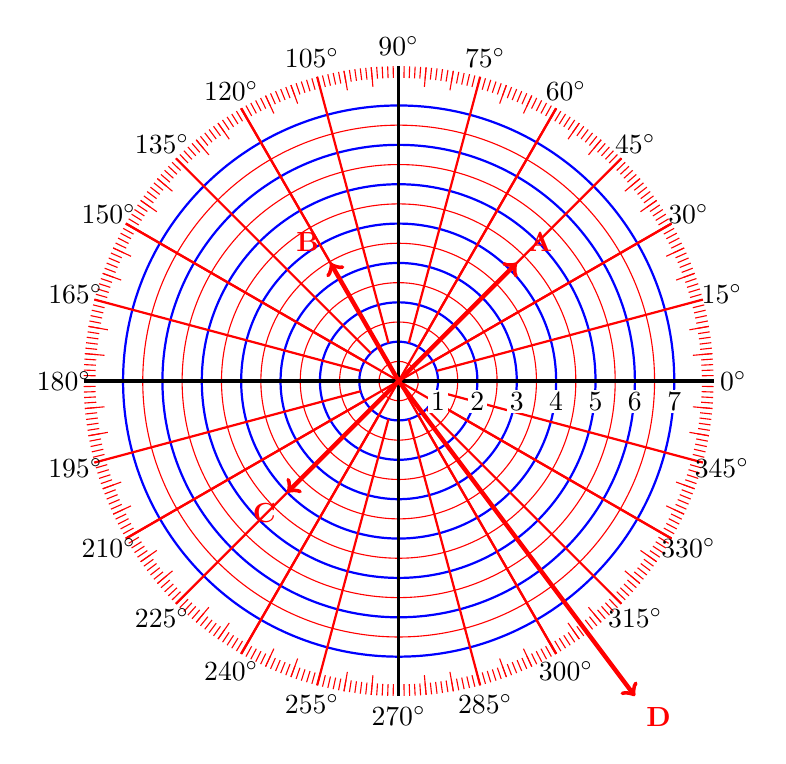
\begin{tikzpicture}[scale=0.5]
        %Circles
        \foreach \r in {1, 2,...,7}
          \draw[blue, thick] (0,0) circle (\r);
        \foreach \r in {0.5, 1.5,...,7}
          \draw[red, thin] (0,0) circle (\r);
        %1° Rays
        \foreach \a in {0, 1,...,359}
          \draw[red] (\a:7.7) -- (\a:8);
        %5° Rays
        \foreach \a in {0, 5,...,359}
          \draw[red] (\a:7.5) -- (\a:8);
        %15° Rays
        \foreach \a in {0, 15,...,359}
          \draw[thick,red] (\a:1) -- (\a:8);
        %30° Rays
        \foreach \a in {0, 30,...,359}
          \draw[thick,red] (0, 0) -- (\a:8);
        %Radius labels (background filled white)
        \foreach \r in {1, 2,...,7}
          \draw (\r,0) node[inner sep=1pt,below=3pt,rectangle,fill=white] {$\r$};
        %Main rays
        \foreach \a in {0, 90,...,359}
          \draw[very thick] (0, 0) -- (\a:8);
        %Angle labels
        \foreach \a in {0, 15,...,359}
          \draw (\a: 8.5) node {$\a^\circ$};
        %Central point
        \draw[->, ultra thick, red] (0,0) -- (xyz polar cs:angle=45,radius={3*sqrt(2)}) node[above right] {\bf A};
        \draw[->, ultra thick, red] (0,0) -- (xyz polar cs:angle=120,radius={2*sqrt(3)}) node[above left] {\bf B};
        \draw[->, ultra thick, red] (0,0) -- (xyz polar cs:angle=225,radius=4) node[below left] {\bf C};
        \draw[->, ultra thick, red] (0,0) -- (xyz polar cs:angle=-53.13,radius=10) node[below right] {\bf D};
      \end{tikzpicture}
    \caption{Exemple de figura amb tikz.}
    \label{fig:polar}
    \end{figure}
    
Figure~\ref{fig:polar} is an example of a figure generated with the tikz library. 


\clearpage
%%%%%%%%%%%%%%%%%%%%%%%%%%%%%%%%%%%%
\section{Results}

In an ordered way, explain the results you have obtained here. This should include a collection of figures, tables, schemas, etc that support the claims that you are obtainig such results. The captions of your figures and tables are as important as the text, and they need to explain "the story" you want to use to demonstrate the claims you do in the project.

Some Equations:
\begin{align*}
    f(x) &= x^2\\
    g(x) &= \frac{1}{x}\\
    F(x) &= \int^a_b \frac{1}{3}x^3
  \end{align*}

Or the vectorial expression of a line in $\mathbb{R}^2$ that goes through point $P(5,-4)$ with a direction parallel to the vector $\vec{v}=(-3,2)$ can be written as:
  \[
  \begin{pmatrix}x\\y\end{pmatrix}=
  \begin{pmatrix}x_0\\y_0\end{pmatrix}+
  t\begin{pmatrix}v_1\\v_2\end{pmatrix}
\]
with its parametric expression:
\begin{equation}
\systeme[t]{x=x_0+t v_1, y=y_0+t v_2}
\label{eq:eq1}
\end{equation}
In Eq.~\ref{eq:eq1} $(x_0,y_0)$ is a point in the line and $\vec{v}=(v_1,v_2)$ is its generating vector. Here:
\[
\systeme[t]{x=5-3t, y=-4+2t}
\]



\clearpage
%%%%%%%%%%%%%%%%%%%%%%%%%%%%%%%%%%%%
\section{Discussion}

Now it is time to put everything together ad to describe how well your results explain your hypothesis through the fullfilling of your objectives. Although everybody likes explaining successful stories, it is equally valid to explian how the project did not succeed in its objectives or in demonstratying its hypothesis as a whole. All comes with the extra perk of opening new questions and facilitating the development of new good research.

\begin{table}
\caption{Example of a  table}
\label{tab:taula}
\begin{tabular}{|c|c|c|c|}
    \hline
    \thead{Sistema} & \thead{$(A|B)$} & Solucions & Rangs\\
    \hline
    $\begin{array}{c}10x+12y=120\\0x+0y=0\end{array}$&
    $\begin{pmatrix}10&12&\vrule&120\\0&0&\vrule&0\end{pmatrix}$&
    $\begin{array}{rcl}x&=&\lambda\\y&=&\frac{120-10\lambda}{12}\end{array}$&
    $\begin{array}{rcl}rg(A)&=&1\\rg(A|B)&=&1\end{array}$
    \\
    \hline
    $\begin{array}{c}10x+12y=120\\10x+12y=120\end{array}$&
    $\begin{pmatrix}10&12&\vrule&120\\10&12&\vrule&120\end{pmatrix}$&
    $\begin{array}{rcl}x&=&\lambda\\y&=&\frac{120-10\lambda}{12}\end{array}$&
    $\begin{array}{rcl}rg(A)&=&1\\rg(A|B)&=&1\end{array}$
    \\
    \hline
    $\begin{array}{c}10x+12y=120\\5x+6y=60\end{array}$&
    $\begin{pmatrix}10&12&\vrule&120\\5&6&\vrule&60\end{pmatrix}$&
    $\begin{array}{rcl}x&=&\lambda\\y&=&\frac{120-10\lambda}{12}\end{array}$&
    $\begin{array}{rcl}rg(A)&=&1\\rg(A|B)&=&1\end{array}$
    \\
    \hline
    $\begin{array}{c}10x+12y=120\\1x+y=10\end{array}$&
    $\begin{pmatrix}10&12&\vrule&120\\5&6&\vrule&10\end{pmatrix}$&
    $\begin{array}{rcl}x&=&0\\y&=&10\end{array}$&
    $\begin{array}{rcl}rg(A)&=&2\\rg(A|B)&=&2\end{array}$
    \\
    \hline
    $\begin{array}{c}10x+12y=120\\10x+12y=100\end{array}$&
    $\begin{pmatrix}10&12&\vrule&120\\10&12&\vrule&100\end{pmatrix}$&
    No té solució&
    $\begin{array}{rcl}rg(A)&=&1\\rg(A|B)&=&2\end{array}$
    \\
    \hline
  \end{tabular}


\end{table}
Table~\ref{tab:taula} is an example of a table containing equations as well.

\clearpage
%%%%%%%%%%%%%%%%%%%%%%%%%%%%%%%%%%%%
\section{Conclusions}

This section can be merged with the preious one, eventually, and summarizes the main findings of the article.


\clearpage
\section{References}

\clearpage
%%%%%%%%%%%%%%%%%%%%%%%%%%%%%%%%%%%%

%% bibliography
\bibliographystyle{plain}
\bibliography{references}

\section{Annexes}
\subsection{Annex 1}
%%%%%%%%%%%%%%%%%%%%%%%%%%%%%%%%%%%%

\end{document}
